\documentclass{beamer}
\usepackage[utf8]{inputenc} 
\usepackage[T1]{fontenc}
\usepackage[francais]{babel}
\usepackage{lmodern}

\usetheme{Darmstadt}
\title[Présentation - MonsterShip]{Présentation - MonsterShip}
\subtitle[\dots]{Pourquoi il vous le faut absolument !}
\author[Olivier - Kevin - Maxime - Antoine]{\bsc{Boissard} Olivier - \bsc{Boulala} Kevin\\\bsc{Dubois} Maxime - \bsc{Lavier} Antoine}
\institute[UFR ST]{UFR ST - Besançon\\Projet de PAD}
\date{\today}

\begin{document}
	\frame{\titlepage}
	
	\section*{Sommaire}
		\begin{frame}
			\frametitle{Sommaire}
			\tableofcontents
		\end{frame}
		
	\section{Contexte}
		\begin{frame}
			\frametitle{Contexte}
			\begin{block}{Données}
				\begin{itemize}
					\item $A$ = Marché du jeu de stratégie spatiale qui s'essouffle
					\item $B$ = Idée révolutionnaire et fortement lucrative
					\item $C$ = Des milliers d'heures de jeu en perspective
					\item $D$ = Un jeu entièrement gratuit (ou presque)
					\item $E$ = Vise le grand public, de l'école primaire à la maison de retraite
				\end{itemize}
			\end{block}
			
			\begin{alertblock}{Résultat}
				\[
					A + B + C + D + E = MonsterShip
				\]
			\end{alertblock}
		\end{frame}
		
	\section{L'univers de MonsterShip}
		\begin{frame}
			\frametitle{Bienvenue en orbite de Sagittarius A*}
			\begin{block}{Incarnez ce que vous êtes}
				\begin{itemize}
					\item Un mercenaire avide de missions
					\item Un capitaine de vaisseau en quête de fortune
					\item Un jeune femmes en détresse
					\item Un programmeur spécialisé PLT-Scheme
					\item ...
				\end{itemize}
			\end{block}
			
			\begin{block}{Avec sous votre contrôle}
				\begin{itemize}
					\item Un équipage dévoué composé de monstres
					\item Un équipage dévoué et prêt à mourir pour vous
					\item Un équipage dévoué et prêt à ne faire qu'un avec le vaisseau
					\item Un vaisseau composé d'un équipage dévoué (et sacrifié)
					\item Divers armes et équipements composés d'un équipage dévoué
				\end{itemize}
			\end{block}
		\end{frame}
		
		\begin{frame}
			\frametitle{Description du jeu}
			\begin{block}{Quelques mots sur MonsterShip}
				\begin{itemize}
					\item Space Opera
					\item Inscription gratuite
					\item Possibilité d'achats d'améliorations
					\item Contrôle d'un vaisseau et de son équipage
					\item Ressource première = équipage du vaisseau
					\item Déplacements sur une map
					\item Interactions avec des planètes
					\item Interactions avec les autres joueurs
				\end{itemize}
			\end{block}
		\end{frame}
		
	\section{Partie technique}
		\begin{frame}
			\frametitle{La partie cachée de l'iceberg}
			\begin{block}{Quelques choix techniques}
				\begin{itemize}
					\item J2EE
					\item Serveur JBoss (WildFly)
					\item API REST \& Javascript
				\end{itemize}
				Nous vous montrerons à quoi peut bien ressembler une API REST à la pointe de la technologie lors de la démonstration
			\end{block}
		\end{frame}
	
	\section{ATTENTION !!}
		\begin{frame}
			\frametitle{VOTRE ATTENTION SVP !!!}
			\begin{alertblock}{WARNING}
				LA SUITE CONTIENT LES SREENSHOTS QUE VOUS ATTENDEZ TOUS, EN AVANT-PREMIERE MONDIALE !!!
			\end{alertblock}
		\end{frame}
		
	\section{Jeu}
		\begin{frame}
		\frametitle{Connexion de l'utilisateur}
			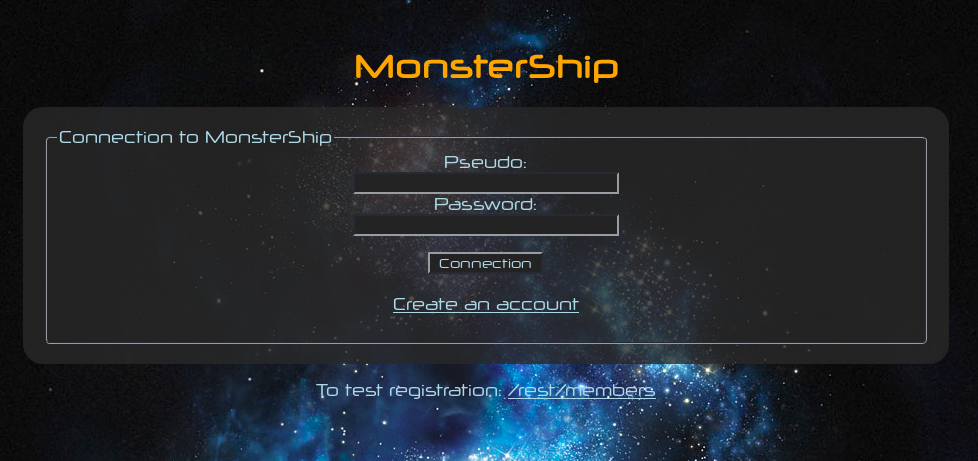
\includegraphics[width=1\textwidth]{images/connexion.png} 
		\end{frame}
		
		\begin{frame}
		\frametitle{Inscription d'un nouvel utilisateur}
			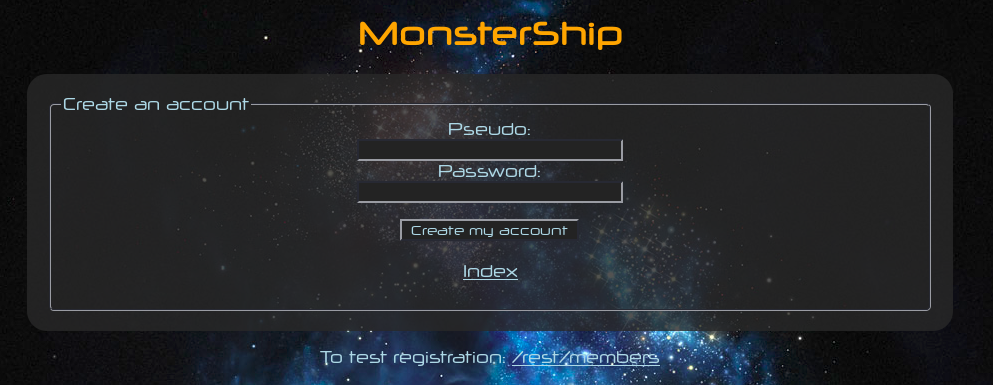
\includegraphics[width=1\textwidth]{images/inscription.png} 
		\end{frame}
		
		\begin{frame}
		\frametitle{Map du jeu}
			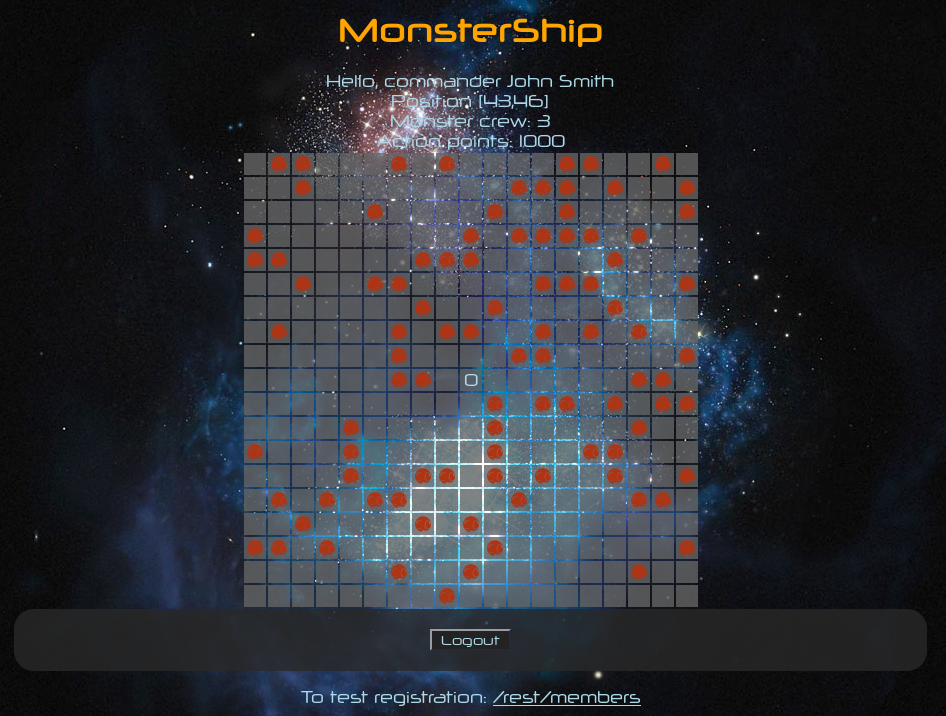
\includegraphics[width=1\textwidth]{images/home.png} 
		\end{frame}
		
	\section{Démo}
	  \begin{frame}
	    \begin{center}
        {\Huge Lançons \href{http://localhost:8080/monstership-web/index.xhtml}{MonsterShip}}
	    \end{center}
	  \end{frame}
		
\end{document}
